% Created by tikzDevice version 0.9 on 2015-12-20 19:43:16
% !TEX encoding = UTF-8 Unicode
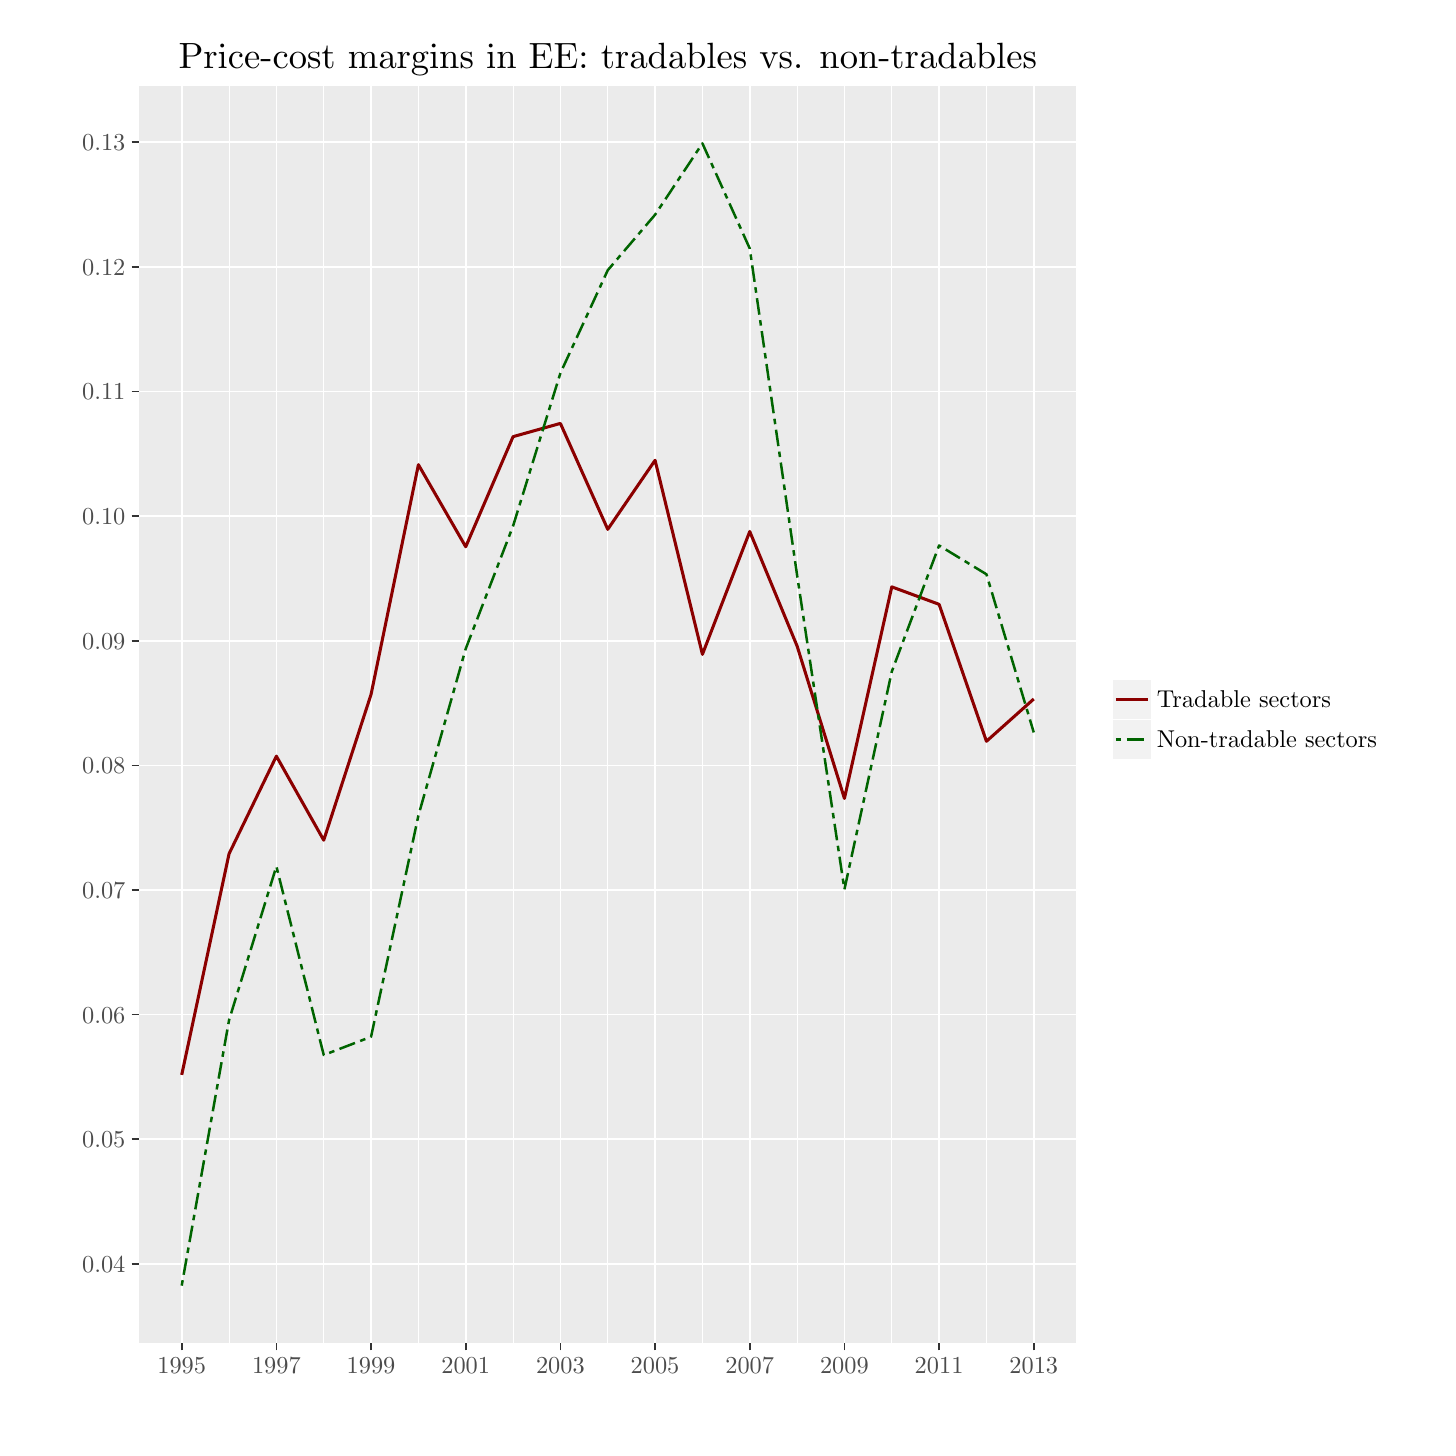
\begin{tikzpicture}[x=1pt,y=1pt]
\definecolor{fillColor}{RGB}{255,255,255}
\path[use as bounding box,fill=fillColor,fill opacity=0.00] (0,0) rectangle (505.89,505.89);
\begin{scope}
\path[clip] (  0.00,  0.00) rectangle (505.89,505.89);
\definecolor{drawColor}{RGB}{255,255,255}
\definecolor{fillColor}{RGB}{255,255,255}

\path[draw=drawColor,line width= 0.6pt,line join=round,line cap=round,fill=fillColor] (  0.00,  0.00) rectangle (505.89,505.89);
\end{scope}
\begin{scope}
\path[clip] ( 40.27, 30.69) rectangle (378.95,484.70);
\definecolor{fillColor}{gray}{0.92}

\path[fill=fillColor] ( 40.27, 30.69) rectangle (378.95,484.70);
\definecolor{drawColor}{RGB}{255,255,255}

\path[draw=drawColor,line width= 0.3pt,line join=round] ( 72.77, 30.69) --
	( 72.77,484.70);

\path[draw=drawColor,line width= 0.3pt,line join=round] (106.98, 30.69) --
	(106.98,484.70);

\path[draw=drawColor,line width= 0.3pt,line join=round] (141.19, 30.69) --
	(141.19,484.70);

\path[draw=drawColor,line width= 0.3pt,line join=round] (175.40, 30.69) --
	(175.40,484.70);

\path[draw=drawColor,line width= 0.3pt,line join=round] (209.61, 30.69) --
	(209.61,484.70);

\path[draw=drawColor,line width= 0.3pt,line join=round] (243.82, 30.69) --
	(243.82,484.70);

\path[draw=drawColor,line width= 0.3pt,line join=round] (278.03, 30.69) --
	(278.03,484.70);

\path[draw=drawColor,line width= 0.3pt,line join=round] (312.24, 30.69) --
	(312.24,484.70);

\path[draw=drawColor,line width= 0.3pt,line join=round] (346.45, 30.69) --
	(346.45,484.70);

\path[draw=drawColor,line width= 0.6pt,line join=round] ( 40.27, 59.17) --
	(378.95, 59.17);

\path[draw=drawColor,line width= 0.6pt,line join=round] ( 40.27,104.21) --
	(378.95,104.21);

\path[draw=drawColor,line width= 0.6pt,line join=round] ( 40.27,149.25) --
	(378.95,149.25);

\path[draw=drawColor,line width= 0.6pt,line join=round] ( 40.27,194.29) --
	(378.95,194.29);

\path[draw=drawColor,line width= 0.6pt,line join=round] ( 40.27,239.32) --
	(378.95,239.32);

\path[draw=drawColor,line width= 0.6pt,line join=round] ( 40.27,284.36) --
	(378.95,284.36);

\path[draw=drawColor,line width= 0.6pt,line join=round] ( 40.27,329.40) --
	(378.95,329.40);

\path[draw=drawColor,line width= 0.6pt,line join=round] ( 40.27,374.44) --
	(378.95,374.44);

\path[draw=drawColor,line width= 0.6pt,line join=round] ( 40.27,419.48) --
	(378.95,419.48);

\path[draw=drawColor,line width= 0.6pt,line join=round] ( 40.27,464.52) --
	(378.95,464.52);

\path[draw=drawColor,line width= 0.6pt,line join=round] ( 55.66, 30.69) --
	( 55.66,484.70);

\path[draw=drawColor,line width= 0.6pt,line join=round] ( 89.87, 30.69) --
	( 89.87,484.70);

\path[draw=drawColor,line width= 0.6pt,line join=round] (124.08, 30.69) --
	(124.08,484.70);

\path[draw=drawColor,line width= 0.6pt,line join=round] (158.29, 30.69) --
	(158.29,484.70);

\path[draw=drawColor,line width= 0.6pt,line join=round] (192.50, 30.69) --
	(192.50,484.70);

\path[draw=drawColor,line width= 0.6pt,line join=round] (226.71, 30.69) --
	(226.71,484.70);

\path[draw=drawColor,line width= 0.6pt,line join=round] (260.92, 30.69) --
	(260.92,484.70);

\path[draw=drawColor,line width= 0.6pt,line join=round] (295.13, 30.69) --
	(295.13,484.70);

\path[draw=drawColor,line width= 0.6pt,line join=round] (329.34, 30.69) --
	(329.34,484.70);

\path[draw=drawColor,line width= 0.6pt,line join=round] (363.55, 30.69) --
	(363.55,484.70);
\definecolor{drawColor}{RGB}{139,0,0}

\path[draw=drawColor,line width= 1.1pt,line join=round] ( 55.66,127.49) --
	( 72.77,207.37) --
	( 89.87,242.65) --
	(106.98,212.28) --
	(124.08,264.96) --
	(141.19,347.97) --
	(158.29,318.31) --
	(175.40,358.10) --
	(192.50,362.89) --
	(209.61,324.61) --
	(226.71,349.56) --
	(243.82,279.44) --
	(260.92,323.83) --
	(278.03,282.44) --
	(295.13,227.37) --
	(312.24,303.82) --
	(329.34,297.51) --
	(346.45,248.02) --
	(363.55,263.31);
\definecolor{drawColor}{RGB}{0,100,0}

\path[draw=drawColor,line width= 0.9pt,dash pattern=on 2pt off 2pt on 6pt off 2pt ,line join=round] ( 55.66, 51.32) --
	( 72.77,147.27) --
	( 89.87,202.83) --
	(106.98,134.65) --
	(124.08,141.25) --
	(141.19,221.19) --
	(158.29,281.46) --
	(175.40,325.83) --
	(192.50,381.06) --
	(209.61,418.24) --
	(226.71,438.29) --
	(243.82,464.06) --
	(260.92,426.08) --
	(278.03,308.04) --
	(295.13,194.49) --
	(312.24,273.20) --
	(329.34,318.78) --
	(346.45,308.37) --
	(363.55,251.21);
\end{scope}
\begin{scope}
\path[clip] (  0.00,  0.00) rectangle (505.89,505.89);
\definecolor{drawColor}{gray}{0.30}

\node[text=drawColor,anchor=base east,inner sep=0pt, outer sep=0pt, scale=  0.88] at ( 35.32, 56.14) {0.04};

\node[text=drawColor,anchor=base east,inner sep=0pt, outer sep=0pt, scale=  0.88] at ( 35.32,101.18) {0.05};

\node[text=drawColor,anchor=base east,inner sep=0pt, outer sep=0pt, scale=  0.88] at ( 35.32,146.22) {0.06};

\node[text=drawColor,anchor=base east,inner sep=0pt, outer sep=0pt, scale=  0.88] at ( 35.32,191.25) {0.07};

\node[text=drawColor,anchor=base east,inner sep=0pt, outer sep=0pt, scale=  0.88] at ( 35.32,236.29) {0.08};

\node[text=drawColor,anchor=base east,inner sep=0pt, outer sep=0pt, scale=  0.88] at ( 35.32,281.33) {0.09};

\node[text=drawColor,anchor=base east,inner sep=0pt, outer sep=0pt, scale=  0.88] at ( 35.32,326.37) {0.10};

\node[text=drawColor,anchor=base east,inner sep=0pt, outer sep=0pt, scale=  0.88] at ( 35.32,371.41) {0.11};

\node[text=drawColor,anchor=base east,inner sep=0pt, outer sep=0pt, scale=  0.88] at ( 35.32,416.45) {0.12};

\node[text=drawColor,anchor=base east,inner sep=0pt, outer sep=0pt, scale=  0.88] at ( 35.32,461.49) {0.13};
\end{scope}
\begin{scope}
\path[clip] (  0.00,  0.00) rectangle (505.89,505.89);
\definecolor{drawColor}{gray}{0.20}

\path[draw=drawColor,line width= 0.6pt,line join=round] ( 37.52, 59.17) --
	( 40.27, 59.17);

\path[draw=drawColor,line width= 0.6pt,line join=round] ( 37.52,104.21) --
	( 40.27,104.21);

\path[draw=drawColor,line width= 0.6pt,line join=round] ( 37.52,149.25) --
	( 40.27,149.25);

\path[draw=drawColor,line width= 0.6pt,line join=round] ( 37.52,194.29) --
	( 40.27,194.29);

\path[draw=drawColor,line width= 0.6pt,line join=round] ( 37.52,239.32) --
	( 40.27,239.32);

\path[draw=drawColor,line width= 0.6pt,line join=round] ( 37.52,284.36) --
	( 40.27,284.36);

\path[draw=drawColor,line width= 0.6pt,line join=round] ( 37.52,329.40) --
	( 40.27,329.40);

\path[draw=drawColor,line width= 0.6pt,line join=round] ( 37.52,374.44) --
	( 40.27,374.44);

\path[draw=drawColor,line width= 0.6pt,line join=round] ( 37.52,419.48) --
	( 40.27,419.48);

\path[draw=drawColor,line width= 0.6pt,line join=round] ( 37.52,464.52) --
	( 40.27,464.52);
\end{scope}
\begin{scope}
\path[clip] (  0.00,  0.00) rectangle (505.89,505.89);
\definecolor{drawColor}{gray}{0.20}

\path[draw=drawColor,line width= 0.6pt,line join=round] ( 55.66, 27.94) --
	( 55.66, 30.69);

\path[draw=drawColor,line width= 0.6pt,line join=round] ( 89.87, 27.94) --
	( 89.87, 30.69);

\path[draw=drawColor,line width= 0.6pt,line join=round] (124.08, 27.94) --
	(124.08, 30.69);

\path[draw=drawColor,line width= 0.6pt,line join=round] (158.29, 27.94) --
	(158.29, 30.69);

\path[draw=drawColor,line width= 0.6pt,line join=round] (192.50, 27.94) --
	(192.50, 30.69);

\path[draw=drawColor,line width= 0.6pt,line join=round] (226.71, 27.94) --
	(226.71, 30.69);

\path[draw=drawColor,line width= 0.6pt,line join=round] (260.92, 27.94) --
	(260.92, 30.69);

\path[draw=drawColor,line width= 0.6pt,line join=round] (295.13, 27.94) --
	(295.13, 30.69);

\path[draw=drawColor,line width= 0.6pt,line join=round] (329.34, 27.94) --
	(329.34, 30.69);

\path[draw=drawColor,line width= 0.6pt,line join=round] (363.55, 27.94) --
	(363.55, 30.69);
\end{scope}
\begin{scope}
\path[clip] (  0.00,  0.00) rectangle (505.89,505.89);
\definecolor{drawColor}{gray}{0.30}

\node[text=drawColor,anchor=base,inner sep=0pt, outer sep=0pt, scale=  0.88] at ( 55.66, 19.68) {1995};

\node[text=drawColor,anchor=base,inner sep=0pt, outer sep=0pt, scale=  0.88] at ( 89.87, 19.68) {1997};

\node[text=drawColor,anchor=base,inner sep=0pt, outer sep=0pt, scale=  0.88] at (124.08, 19.68) {1999};

\node[text=drawColor,anchor=base,inner sep=0pt, outer sep=0pt, scale=  0.88] at (158.29, 19.68) {2001};

\node[text=drawColor,anchor=base,inner sep=0pt, outer sep=0pt, scale=  0.88] at (192.50, 19.68) {2003};

\node[text=drawColor,anchor=base,inner sep=0pt, outer sep=0pt, scale=  0.88] at (226.71, 19.68) {2005};

\node[text=drawColor,anchor=base,inner sep=0pt, outer sep=0pt, scale=  0.88] at (260.92, 19.68) {2007};

\node[text=drawColor,anchor=base,inner sep=0pt, outer sep=0pt, scale=  0.88] at (295.13, 19.68) {2009};

\node[text=drawColor,anchor=base,inner sep=0pt, outer sep=0pt, scale=  0.88] at (329.34, 19.68) {2011};

\node[text=drawColor,anchor=base,inner sep=0pt, outer sep=0pt, scale=  0.88] at (363.55, 19.68) {2013};
\end{scope}
\begin{scope}
\path[clip] (  0.00,  0.00) rectangle (505.89,505.89);
\definecolor{fillColor}{RGB}{255,255,255}

\path[fill=fillColor] (387.49,237.16) rectangle (491.85,278.22);
\end{scope}
\begin{scope}
\path[clip] (  0.00,  0.00) rectangle (505.89,505.89);
\definecolor{drawColor}{RGB}{255,255,255}
\definecolor{fillColor}{gray}{0.95}

\path[draw=drawColor,line width= 0.6pt,line join=round,line cap=round,fill=fillColor] (391.75,255.89) rectangle (406.21,270.34);
\end{scope}
\begin{scope}
\path[clip] (  0.00,  0.00) rectangle (505.89,505.89);
\definecolor{drawColor}{RGB}{139,0,0}

\path[draw=drawColor,line width= 1.1pt,line join=round] (393.20,263.11) -- (404.76,263.11);
\end{scope}
\begin{scope}
\path[clip] (  0.00,  0.00) rectangle (505.89,505.89);
\definecolor{drawColor}{RGB}{255,255,255}
\definecolor{fillColor}{gray}{0.95}

\path[draw=drawColor,line width= 0.6pt,line join=round,line cap=round,fill=fillColor] (391.75,241.43) rectangle (406.21,255.89);
\end{scope}
\begin{scope}
\path[clip] (  0.00,  0.00) rectangle (505.89,505.89);
\definecolor{drawColor}{RGB}{0,100,0}

\path[draw=drawColor,line width= 0.9pt,dash pattern=on 2pt off 2pt on 6pt off 2pt ,line join=round] (393.20,248.66) -- (404.76,248.66);
\end{scope}
\begin{scope}
\path[clip] (  0.00,  0.00) rectangle (505.89,505.89);
\definecolor{drawColor}{RGB}{0,0,0}

\node[text=drawColor,anchor=base west,inner sep=0pt, outer sep=0pt, scale=  0.88] at (408.01,260.08) {Tradable sectors};
\end{scope}
\begin{scope}
\path[clip] (  0.00,  0.00) rectangle (505.89,505.89);
\definecolor{drawColor}{RGB}{0,0,0}

\node[text=drawColor,anchor=base west,inner sep=0pt, outer sep=0pt, scale=  0.88] at (408.01,245.63) {Non-tradable sectors};
\end{scope}
\begin{scope}
\path[clip] (  0.00,  0.00) rectangle (505.89,505.89);
\definecolor{drawColor}{RGB}{0,0,0}

\node[text=drawColor,anchor=base,inner sep=0pt, outer sep=0pt, scale=  1.32] at (209.61,491.30) {Price-cost margins in EE: tradables vs. non-tradables};
\end{scope}
\end{tikzpicture}
